\documentclass[tikz,border=10pt]{standalone}
\usetikzlibrary{calc}

\tikzset{
    car/.pic={
        % Wheels
        \fill[black!85, rounded corners=0.5pt] (-0.9, 0.6) rectangle (-0.5, 1.1);
        \fill[black!85, rounded corners=0.5pt] (0.5, 0.6) rectangle (0.9, 1.1);
        \fill[black!85, rounded corners=0.5pt] (-0.9, -1.1) rectangle (-0.5, -0.6);
        \fill[black!85, rounded corners=0.5pt] (0.5, -1.1) rectangle (0.9, -0.6);
        % Main Body
        \draw[fill=gray!15, rounded corners=4pt, thin] (-0.7,-1.2) rectangle (0.7,1.2);
    }
}

\begin{document}
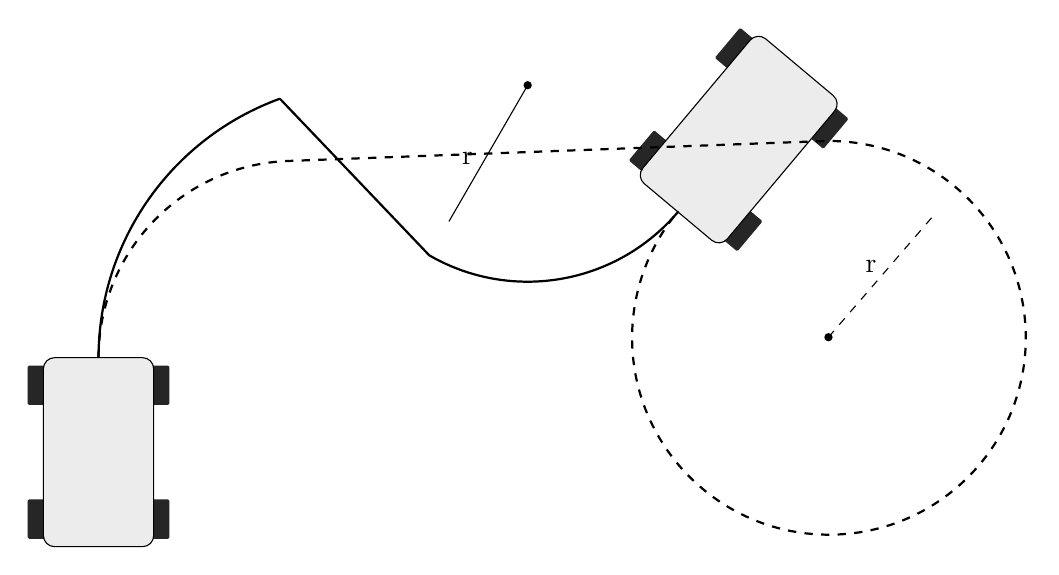
\begin{tikzpicture}[scale=1.0, >=stealth]

    % 1. Start Pose (Car 1)
    % Positioned at origin, facing UP (90 degrees in standard polar)
    \pic[rotate=0] at (0,0) {car};

    % 2. End Pose (Car 2)
    % Placed to perfectly align with the terminal tangent of the true geometric arcs
    \pic[rotate=-40] at (8.13, 3.97) {car};

    % ==========================================
    % Reeds-Shepp Path (Solid Line: C - S - C)
    % Constructed strictly with true circular arcs and straight lines
    % ==========================================
    % Curve 1: Forward right turn to cusp (radius = 3.5)
    \draw[thick] (0, 1.2) arc (180:110:3.5) coordinate (cusp);
    
    % Straight segment: Reversing
    \draw[thick] (cusp) -- (4.2, 2.5) coordinate (rs_mid);
    
    % Curve 2: Reversing left turn into Car 2 (radius = 2.5)
    \draw[thick] (rs_mid) arc (-120:-40:2.5);

    % True radius line and center point for Reeds-Shepp curve (second arc)
    \fill (5.45, 4.66) circle (1.5pt);
    \draw (5.45, 4.66) -- (4.45, 2.93) node[midway, left, xshift=-2pt, yshift=-2pt] {r};

    % ==========================================
    % Dubins Path (Dashed Line: R - S - R)
    % Constructed strictly with true circular arcs and straight tangent lines
    % ==========================================
    % Right turn -> straight tangent line -> large right turn loop
    \draw[thick, dashed] (0, 1.2) arc (180:92.2:2.5) 
        -- (9.18, 3.95) 
        arc (92.2:-220:2.5);

    % True radius line and center point for the terminal Dubins loop
    \fill (9.27, 1.46) circle (1.5pt);
    \draw[dashed] (9.27, 1.46) -- (10.6, 3.0) node[midway, above left, xshift=2pt, yshift=-2pt] {r};

\end{tikzpicture}
\end{document}